\documentclass[10pt]{article}

\def\Type{LessonCaelan}
\def\TypeNum{Lesson 17}
\def\TypeTitle{Antiderivatives \& Indefinite Integrals \\Solutions }
\def\Semester{Fall 2021} %Not Used 
\def\Course{MATH 1190 \& 1210}
\def\Targets{  \bf\color{Fuchsia}I3 }

\usepackage{preambleDJ}

%\usepackage{ragged2e}


%%%%%%%%%%%% BEGIN DOCUMENT %%%%%%%%%%%%%%%
%%%%%%%%%%%% BEGIN DOCUMENT %%%%%%%%%%%%%%%
%%%%%%%%%%%% BEGIN DOCUMENT %%%%%%%%%%%%%%%
%%%%%%%%%%%% BEGIN DOCUMENT %%%%%%%%%%%%%%%
%%%%%%%%%%%% BEGIN DOCUMENT %%%%%%%%%%%%%%%




\begin{document}

\pagestyle{otherpages}
\thispagestyle{firstpage}
\vs{.7}

\textbf{Intended Learning Outcomes}
After this lesson, you will be able to 

\begin{itemize}
    \item Find antiderivatives of power and exponential functions. (\target{I3})
    %\item Use graph (and possibly additional information) of a function to deduce information about its antiderivative.
    \item Use algebraic simplification and/or properties of an indefinite integral to find the indefinite integral of a function. (\target{I3})
\end{itemize}

\vspace{-0.6cm}

\hrulefill\\

\blue{\bf Basic Antidifferentiation Rules}

{\bf\color{blue} Fill in the blanks!} Let $F$ and $G$ be antiderivatives of $f$ and $g$, respectively, and let $k$ be a constant.

\begin{itemize}

\item {\bf Definition:} A function $F$ is called an {\bf antiderivative} of $f$ on an interval $I$ if $\unlineb{.5}{F^{\prime}(x)} \;=\; \unlineb{.5}{f(x)}$ for all $x$ in $I$.\\

\item A particular antiderivative of $kf(x)$ is \dotfill $\unlineb{1}{kF(x)}$.\\

\item A particular antiderivative of $f(x)\pm g(x)$ is \dotfill $\unlineb{2}{F(x)\pm G(x)}$.\\

\item The {\bf indefinite integral} of a function is the most general antiderivative of that function: 

\[\dint f(x)\,dx = \unlineb{2}{F(x)+C}\]

\end{itemize}

\

\hrulefill

\

%{\exercise} Use the definition of an antiderivative to respond to the following:\\

%Is $\dfrac{x}{x^2+1}$ an antiderivative of $\dfrac{1-x^2}{(x^2+1)^2}$? Why or why not?

%\vfill
{\bf\color{blue} Warm-up Exercise 1.} Find the following derivatives: Try these on your own. After you have made your attempt, compare notes with your neighbor.\\

\mpageT{.5}{.5}[\hfill]{
        \begin{itemize}
        \item $\ds \dfrac{d}{dx}\left[ x^2\right] = \unlineb{1}{2x}$
        \item $\ds \dfrac{d}{dx}\left[ x^3\right] = \unlineb{1}{3x^2}$
        \item $\ds \dfrac{d}{dx}\left[ x^{5/4}\right] = \unlineb{1}{\dfrac{5}{4}x^{1/4}}$
        \end{itemize}
}{
     \begin{itemize}
        \item $\ds \dfrac{d}{dx}\left[ \frac12x^2\right] = \unlineb{1}{x}$
        \item $\ds \dfrac{d}{dx}\left[ 2x^3\right] = \unlineb{1}{6x^2}$
        \item $\ds \dfrac{d}{dx}\left[ \dfrac45x^{5/4}\right] = \unlineb{1}{x^{1/4}}$
        \end{itemize}
}
\vfill
{\bf\color{blue} Warm-up Exercise 2.} Find the following derivatives: Try these on your own. After you have made your attempt, compare notes with your neighbor.\\
\mpageT{.5}{.5}[\hfill]{
\begin{itemize}
        \item $\ds \dfrac{d}{dx}\left[ \ln(x)\right] = \unlineb{1}{\dfrac{1}{x}}$
        \item $\ds \dfrac{d}{dx}\left[ x^{-1}\right] = \unlineb{1}{-x^{-2}}$
           \item $\ds \dfrac{d}{dx}\left[ 2 e^x\right] = \unlineb{1}{2e^x}$
        \end{itemize}
}{
\begin{itemize}
        \item $\ds \dfrac{d}{dx}\left[ 9\ln(x)\right] = \unlineb{1}{\dfrac{9}{x}}$
        \item $\ds \dfrac{d}{dx}\left[ 2x^{-1}\right] = \unlineb{1}{-2x^{-2}}$
                   \item $\ds \dfrac{d}{dx}\left[ 2 \cdot 3^x\right] = \unlineb{1}{2\cdot 3^x\cdot\ln(3)}$
        \end{itemize}
}

\vfill
\newpage



\blue{\bf Antiderivatives of Power Functions, Exponential Functions, Log Functions and Polynomials}\\

{\exercise}\ltrm{\bf\color{Fuchsia}I3} Find the following antiderivatives. ({\bf Hint 1}: you might ask yourself questions like ``which function has a derivative of $2x$?" when filling in the table. {\bf Hint 2:} Work done on previous page might be a helpful reference.)

\renewcommand{\arraystretch}{2}


\begin{center}
    \begin{tabularx}{6in}{ | C{1} | C{1} || C{1} | C{1} | }
    \hline
    Function & Particular antiderivative & Function & Particular antiderivative\\
    \hline
    $2x$ & $\blue{x^2}$& $6x$ & $\blue{3x^2}$ \\
    \hline
    $3x^2$ & $\blue{x^3}$ & $x^2$ & $\blue{\dfrac{x^3}{3}}$ \\
    \hline
    $\dfrac32x^{1/2}$ & $\blue{x^{3/2}}$ & $6x^{1/2}$ &$\blue{4x^{3/2}}$ \\
    \hline
    $-x^{-2}$ &$\blue{x^{-1}}$ & $2x^{-2}$ &$\blue{2x^{-1}}$ \\
    \hline
    $\dfrac1x$ &$\blue{\ln|x|}$ & $\dfrac{2}{x}$ &$\blue{2\ln|x|}$ \\
    \hline
    $-\dfrac1{x^2}$ &$\blue{x^{-1}}$ & $\dfrac2{x^2}$ &$\blue{2x^{-1}}$ \\
    \hline
    $5e^x$ &$\blue{5e^x}$ & $ 4^x$ &$\blue{\dfrac{1}{\ln(4)} 4^x}$ \\
    \hline
      $x^n$ ($n\not=-1$) &$\blue{\dfrac{x^{n+1}}{n+1}}$ & $x^{-1}$ &$\blue{\ln|x|}$ \\
      \hline
    \end{tabularx}
\end{center}

\vs{.2}

Now, find a particular antiderivative of $\ds f(x)=6x-x^{-2}+6x^{1/2}+\dfrac2x-\dfrac1{x^2}$.\\

\begin{center}
$F(x) = \unlineb{5}{ 3x^2 + x^{-1} + 4x^{3/2} + 2\ln|x| + x^{-1} }$
\end{center}
\vs{.2}
Based on your work above, fill in the following indefinite integral formulas:\\

$\dint x^n\,dx = \underset{\text{assuming }n\not=-1}{\text{\unlineb{1.5}{\dfrac{x^{n+1}}{n+1}+C}}}$
\hfill
$\dint \frac1x\,dx = \unlineb{1.5}{\ln|x|+C}$

\vs{.2}
Find a particular antiderivative of $g(x) =x^2+ \dfrac{3}{2}x^{1/2}+5e^x+4^x$\\
\begin{center}
$G(x) = \unlineb{5}{\ds \frac{x^3}{3}+x^{3/2}+5e^x+\frac{1}{\ln(4)}4^x}$
\end{center}


\vs{.2}
Based on your work above, fill in the following indefinite integral formulas:\\
$\dint e^x\,dx = \unlineb{1.5}{e^x+C}$
\,\hfill
$\dint a^x\,dx =\underset{\text{assuming }a>0\,\&\,a\not=1}{\text{\unlineb{1.5}{\dfrac{1}{\ln(a)} a^x}}}$
\,\hfill
\vs{.2}\\
Finally, find a particular antiderivative of $h(x) = x + x^{-3} + 7x^{1/3} - x^{-1} + \dfrac{1}{\sqrt[3]{x}}\blue{=x+x^{-3}+7x^{1/3}-x^{-1}+x^{-1/3}}$.\\
\begin{center}
$H(x) = \unlineb{5}{\ds \frac{x^2}{2} - \frac{1}{2} x^{-2} + \frac{21}{4}x^{4/3} - \ln|x| + \frac{3}{2}x^{2/3} }$
\end{center}







%%%%%%%%%
\newpage%
%%%%%%%%%


\blue{\bf Summary of Indefinite Integrals}


{\bf\color{blue} Fill in the blanks!}\ltrm{\bf\color{Fuchsia}I3} Assume $k$ is any constant. Furthermore, assume $f$ has antiderivative $F$ and $g$ has antiderivative $G$. Fill in the blanks below to complete the table containing some basic indefinite integrals.

\begin{center}
{\it Integral of a Constant}\\[0.1in]
\begin{tabular}{ r c l}
$\displaystyle\int k\, dx$ & $=$ & $\unlineb{1.75}{kx+C}$
\end{tabular}
\end{center}

\

\begin{center}
{\it Integral of Power Functions}\\[0.1in]
\begin{tabular}{ r c l r c l}
$\displaystyle\int x^n\, dx$ & ${=}$ & $\underset{\text{assuming }n\not=-1}{\text{ $\unlineb{1.75}{\dfrac{x^{n+1}}{n+1}+C}$}}$ & $\displaystyle\int\frac1x\,dx$ & $=$ &  $\unlineb{1.75}{\ln|x|+C}$\\[0.1in]
\end{tabular}
\end{center}

\

\begin{center}
{\it Integral of Exponential Functions}\\[0.1in]
\begin{tabular}{ r c l r c l}
$\displaystyle\int e^x\, dx$ & $=$ &$\unlineb{1.75}{e^x+C}$ & $\displaystyle\int a^x\,dx$ & $=$ & $\underset{\text{assuming }a>0\,\&\,a\not=1}{\text{$\unlineb{1.75}{\dfrac{1}{\ln(a)}a^x+C}$}}$\\[0.1in]
\end{tabular}
\end{center}

\

\begin{center}
{\it Linearity Properties of Indefinite Integrals}\\[0.1in]
\begin{tabular}{ r c l r c l}
$\displaystyle\int \big( f(x) \pm g(x) \big)\, dx$ & $=$ & $\unlineb{1.75}{F(x) \pm G(x)+C}$ & $\displaystyle\int kf(x) \,dx$ & $=$ & $\unlineb{1.75}{kF(x)+C}$\\[0.1in]
\end{tabular}
\end{center}

\

{\exercise}\ltrm{\bf\color{Fuchsia}I3} Find the following indefinite integrals:

\begin{enumerate}

\item[(a)] $\dint \sqrt2 \,dx$
\sol{
$\sqrt{2}x+C$
}



\item[(b)] $\dint \left(\sqrt[3]{u}+4u^{-1}+\frac{1}{u^2}\right)\,du$
\sol{
\al{
\dint \left(\sqrt[3]{u}+4u^{-1}+\frac{1}{u^2}\right)\,du&=\dint \left( u^{1/3}+4u^{-1}+u^{-2}\right)\,du\\
&=\frac{3}{4} u^{4/3} + 4 \ln|u| - u^{-1} + C
}
}

\item[(c)] $\dint \left(\dfrac{y^4-1}{y^2} \right)\,dy$ 
\sol{
\al{
\dint \frac{y^4-1}{y^2} dy 
&= \dint \frac{y^4}{y^2} -\frac{1}{y^2} dy\\
&= \dint y^2 -\frac{1}{y^2} dy\\
&= \frac{y^3}{3} + y^{-1} + C
}
}

\end{enumerate}

%%%%%%%%%
\newpage%
%%%%%%%%%

\ep \ltrm{\bf\color{Fuchsia}I3} Find the following indefinite integrals:

\begin{enumerate}

\item[(a)] $\dint \left(2 - 6t^3 + \dfrac{3}{t^2} - e^t \right)\,dt$
\sol{
\al{
\dint \left(2 - 6t^3 + \dfrac{3}{t^2} - e^t \right)\,dt&=\dint \left(2 - 6t^3 + 3t^{-2} - e^t \right)\,dt\\
&=2t - \frac{3}{2} t^4 - 3 t^{-1} - e^t + C
}
}

\item[(b)] $\dint \dfrac{x^3+x^2-x+1}{2x^2}\,dx$

\sol{
\al{
\dint \frac{x^3+x^2-x+1}{2x^2} dx &= \dint \frac{x^3}{2x^2} + \frac{x^2}{2x^2} - \frac{x}{2x^2} + \frac{1}{2x^2} dx\\
&= \dint \frac{x}{2} + \frac{1}{2} - \frac{1}{2x} + \frac{1}{2x^2} dx\\
&= \frac{x^2}{4} + \frac{x}{2} - \frac{1}{2} \ln|x| - \frac{1}{2}x^{-1} + C
}
}


\item[(c)] $\dint \left( z^2 + \dfrac1{z^2}\right) \left( z - \dfrac{1}{z} \right) \, dz$
\sol{
\al{
\dint \left(z^2 + \frac1{z^2}\right) \left( z - \frac1{z} \right) dz &= \dint \left(z^3   - z + \frac{1}{z} - \frac{1}{z^3}\right) dz\\
&=\dint \left(z^3   - z + \frac{1}{z} - z^{-3}\right) dz\\
&= \frac{z^4}{4} - \frac{1}{2}z^{2} + \ln|z| + \frac{1}{2}z^{-2} + C\\
&= \frac{z^4}{4} - \frac{1}{2}z^{2} + \ln|z| + \frac{1}{2z^2} + C
}
}
\newpage
\ep \ltrm{{\bf\color{RedOrange}A3}} Problem \# $5$ from textbook, section 4.5.\\\\
The management of the UNICO department store has decided to enclose an $800$ ft$^2$ area outside the building for displaying potted plants and flowers.  One side will be formed by the external wall of the store, two sides will be constructed of pine boards and the fourth side will be made of galvanized steel fencing. if the pine board fencing costs $\$6$ per running foot and the steel fencing costs $\$3$ per running foot, determine the dimensions of the enclosure that can be erected at minimum cost.
\graphicsC{unicoLabeled}{3}
\blue{
{\bf Modeling Phase}
We use the variable $x$ to describe the length (in feet) of the plant/flower area and the variable $y$ to describe the width (in feet) of the same area (see Figure 1). Our goal is to minimize the cost.
$$Cost=Cost_{length}+Cost_{width}$$
\itemI{
\item Since the length will be made of galvanized steel fencing with cost of $\$3$ per foot and we're using $x$ feet, $$Cost_{length}=3x.$$
\item Since the each width will be made of pine fencing with cost of $\$6$ per foot and we're using $y$ feet for each side, $$Cost_{width}=6y+6y=12y.$$
}
Thus 
\al{
Cost&=Cost_{length}+Cost_{width}\\
Cost&=3x+12y
}
We are also told that the area is $800$ ft$^2$. Thus
$$A=xy=800.$$
{\bf Calculus Phase}\\
In order to minimize Cost, we need to find critical numbers. This requires finding a derivative. We cannot currently do this since $Cost$ is a function of two variables.  However we can use our area assumption to solve for one variable in terms of the other. In particular
\al{
xy&=800\\
y&=\frac{800}{x}
}
We can update our Cost function
\al{
Cost&=3x+12y\\
&=3x +12 \cdot \frac{800}{x}\\
&=3x+\frac{9600}{x}\\
Cost(x)&=3x+9600x^{-1}\\
\frac{d}{dx}\,Cost&=\frac{d}{dx} \left[ 3x+9600x^{-1}\right] \\
&=3-9600x^{-2}\\
Cost^{\prime}(x)&=3-\frac{9600}{x^2}
}
{\em Finding critical numbers}
\itemI{
\item We note that $Cost^{\prime}(x)$ DNE when $x=0$ due to the division by $0$. Thus $x=0$ is a critical number.
\item We also solve $Cost^{\prime}(x)=0$ to find other critical numbers.
\al{
3-\frac{9600}{x^2}&=0\\
3&=\frac{9600}{x^2}\\
\intertext{Multiply both sides by $x^2$ to get}
3x^2&=9600\\
\intertext{Divide both sides by $3$ to get}
x^2&=\frac{9600}{3}=3200\\
x&=\pm \sqrt{3200}\\
x&\approx \pm 56.57
}
\item We have $3$ critical numbers: $x=-\sqrt{3200}$, $x=0$ and $x=\sqrt{3200}$
\item Since $x$ represents the length in feet, a negative value does not make sense nor does $x=0$. Thus our domain is $0<x<\infty$ and we can ignore critical numbers $x=-\sqrt{3200}$ and $x=0$ since they are not in our domain.  
}
{\em Determining local minimum}
We use the First Derivative Test to determine if we have a local minimum (or not).
\itemI{
\item We choose a value less than $x=\sqrt{3200}$, say $x=1$.
$$Cost^{\prime}(1)=3-\frac{9600}{1^2}=-9597<0$$
\item We choose a value greater than $x=\sqrt{3200}$, say $x=100$.
$$Cost^{\prime}(100)=3-\frac{9600}{(100)^2}=3-\frac{9600}{10000}=3-0.96=2.04>0$$
}
\mpageT{.5}{.5}{
The sign chart on the right captures this information. We see that we have a local minimum. Since we have only one critical number, $x=\sqrt{3200}\approx 56.57$, in our domain $0<x<\infty$, The First Derivative Test for Absolute Extrema says that the local minimum is also the absolute minimum.
}{
\begin{center}
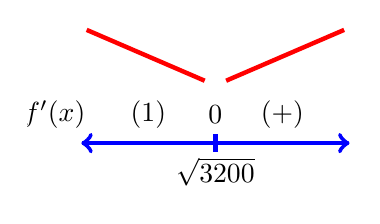
\begin{tikzpicture}
    \begin{axis}[
    	axis x line=none,
	            axis y line=none,
		x label style={anchor=west},
            xlabel={},
            xtick       = {0},
            xticklabels = {$c$},
            y label style={anchor=south},
            ylabel={},
            ytick       = {-6,-4,-2,2,4,6},
            yticklabels = {$-6$,$-4$,$-2$,$2$,$4$,$6$},
            samples     = 320,
            domain      = -2.5:2.5,
            restrict y to domain=-6.5:6.5,
            xmin = -3.5, xmax = 3.5,
            ymin = -6.5, ymax = 6.5,
            width=2.5in, height=2.5in,
            grid=none, grid style=solid
          ]
    \addplot[domain=-2.5:2.5, blue, ultra thick, mark=none, <->]{0)};
   \draw (-3,1) node{$\Large f^{\prime}(x)$};
   \draw[ultra thick, blue] (0,.3)--(0,-.3);
      \draw (0,-1) node{$\sqrt{3200}$};
            \draw (0,1) node{$0$};
            \addplot[domain=-2.4:-.2, red, ultra thick, mark=none, -]{-2*x/2.5+2)};
                        \addplot[domain=0.2:2.4, red, ultra thick, mark=none, -]{2*x/2.5+2)};
                             \draw (-1.25,1) node{\blue{$(1)$}};
                              \draw (1.25,1) node{\blue{$(+)$}};
    \end{axis}
\end{tikzpicture}
\end{center}
}
~\\\\
Lastly, since $\ds y=\frac{800}{x}$, $\ds y=\frac{800}{\sqrt{3200}}\approx 14.14$ feet.

Thus the dimensions of the enclosure that minimize cost are $x=\sqrt{3200}\approx56.57$ feet and $\ds y=\frac{800}{\sqrt{3200}} \approx 14.14$ feet.

}

\end{enumerate}
\end{document}
